The diagram shows twenty congruent circles arranged in three rows and enclosed in a rectangle.  The circles are tangent to one another and to the sides of the rectangle as shown in the diagram.  The ratio of the longer dimension of the rectangle to the shorter dimension can be written as $\frac{1}{2}\left(\sqrt{p}-q\right),$ where $p$ and $q$ are positive integers.  Find $p+q.$

\begin{center}
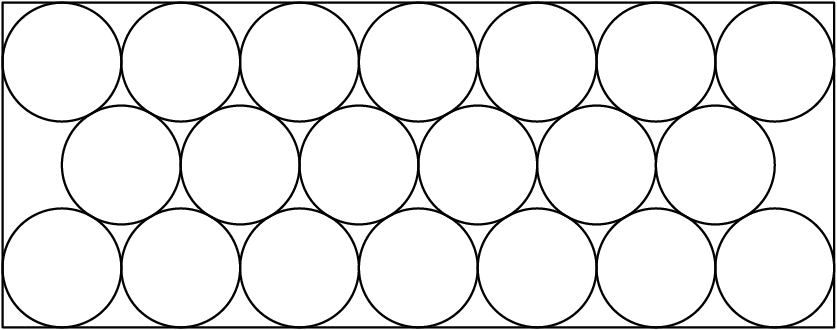
\includegraphics[width = 83.60000000000001mm]{img/fig0.png}
\end{center}